\section{WhyCode Modifications}
\label{section:whycode_modifications}

\subsection{Background}

The WhyCon fiducial marker, shown in Figure \ref{fig:whycon} consists of a white circle inside of a larger black circle.
The identification algorithm is computationally simple:
\begin{itemize}
    \item An input image is searched for white regions.
    \item The detector flood-fills and determines a measure of circularity for each white region.
    \item The detector seeks a black region directly outside of each white region, flood fills it, and determines a measure of circularity for it.
    \item The circularity measures are compared, and the white/black region combination is called a WhyCon marker if it is adequately circular (under projection).
    \item The position of the marker is determined using the pinhole model of a monocular camera with known intrinsic parameters
            (pixel resolution, lens distortion, principal points, focal lengths), and the diameter of the marker.
    \item The major and minor axes of the elliptical regions provide a basis from which to determine the marker's orientation.
\end{itemize}

The WhyCon software's purpose is to determine the pose (position \textit{and} orientation) of detected WhyCon markers
with respect to the camera field of view.
The position of the markers can be determined with centimeter accuracy in most use cases.
However, the full radial symmetry of the WhyCon marker inherently prevents the assignment or recognition
of a ``yaw'' orientation - that is, only two components of the marker's rotation can be determined.

\begin{figure}
    \centering
    
\includegraphics[width=0.16\textwidth]{images/whycon_example.png}
    \caption{WhyCon marker.}
    \label{fig:whycon}
\end{figure}

WhyCode expands on WhyCon to add an ID and yaw orientation to the plain WhyCon marker.
While the majority of the detection algorithm is the same,
an ID is encoded onto the marker in the form of a Manchester encoding that is wrapped around the inner, white circle,
as shown in Figure \ref{fig:whycode_id}.
By sampling along the circle halfway between the white circle and black circle, the detector can determine the ID encoding.
Figure \ref{fig:rotationally_symmetric_whycode_markers} shows potential collisions between WhyCode markers that are
rotationally symmetric but have different IDs.
While it is impossible to distinguish between rotationally symmetric markers, this problem can be overcome by bit-shifting
the ID's binary string to its lowest value in all cases before determining the ID.
This also gives a means of determining a ``yaw origin'' so that the orientation of the marker can be determined in 3 dimensions.

\begin{figure}
    \centering
    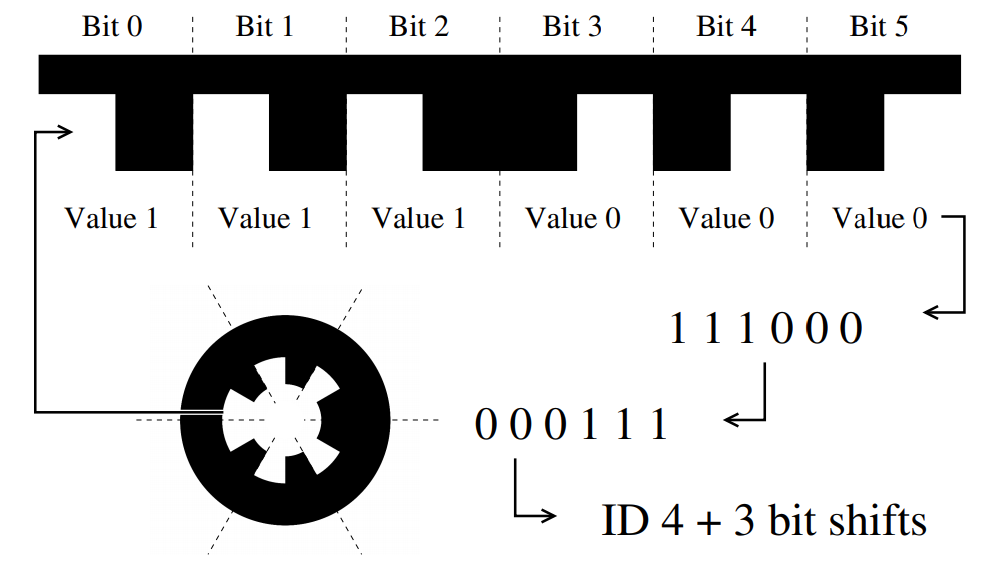
\includegraphics[width=0.4\textwidth]{images/whycode_manchester_explanation.png}
    \caption{WhyCode ID Manchester ``Necklace'' Encoding.}
    \label{fig:whycode_id}
\end{figure}

\begin{figure}
    \centering
    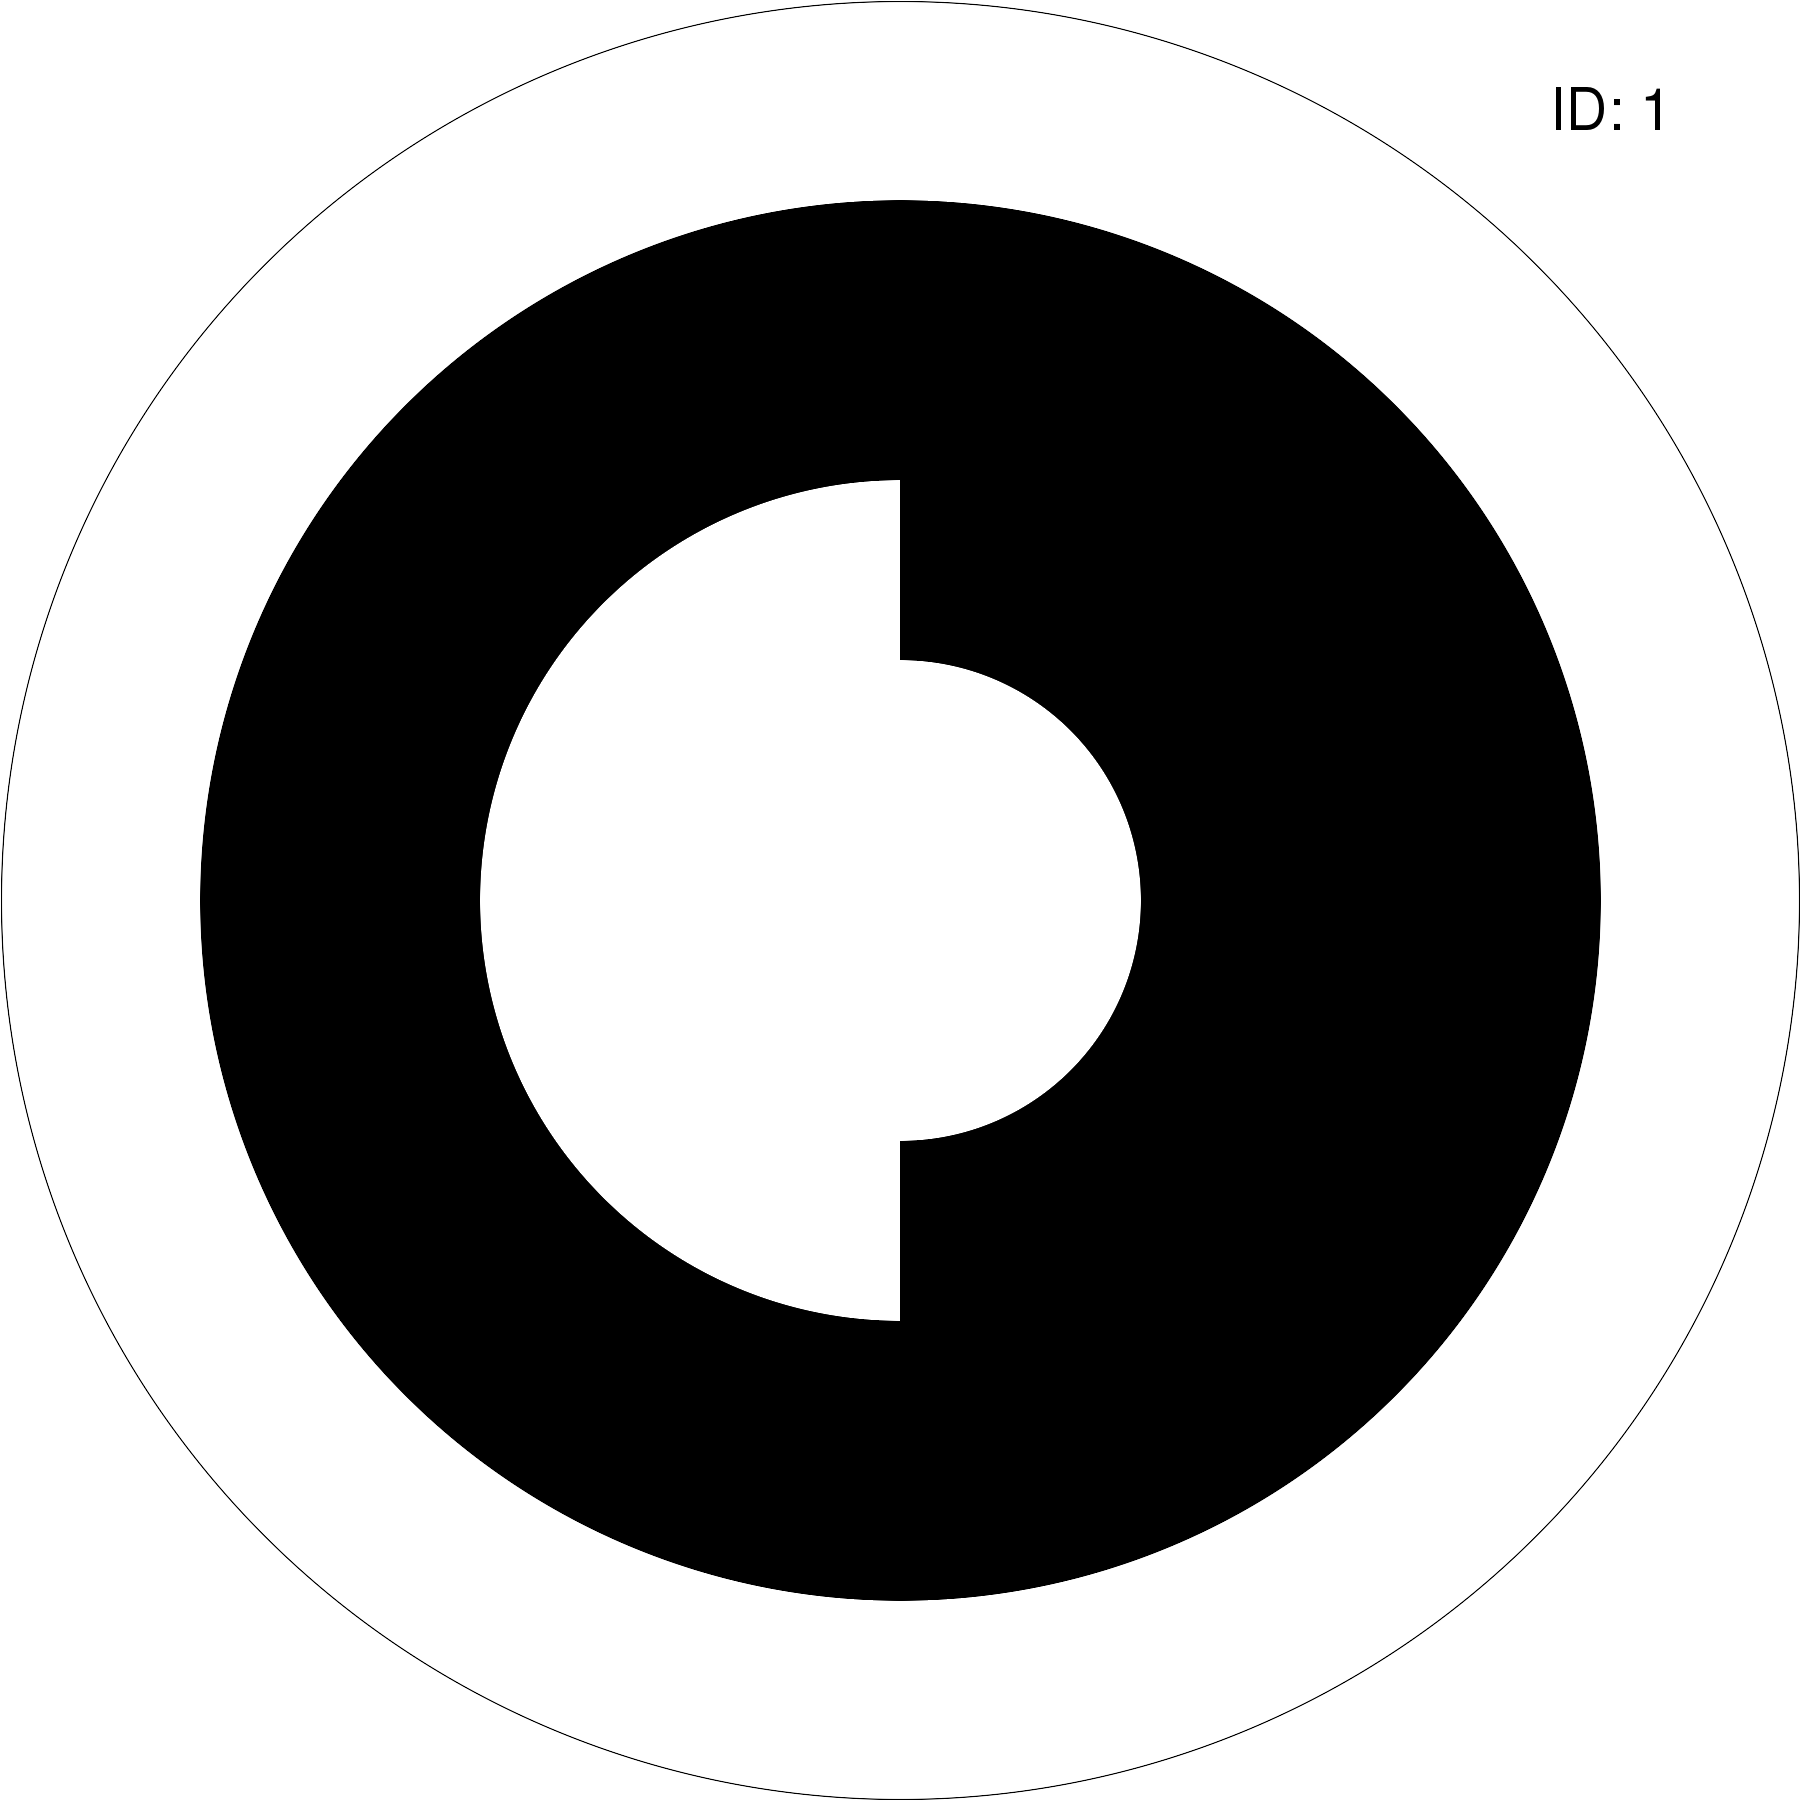
\includegraphics[width=0.2\textwidth]{images/00000001.png}
    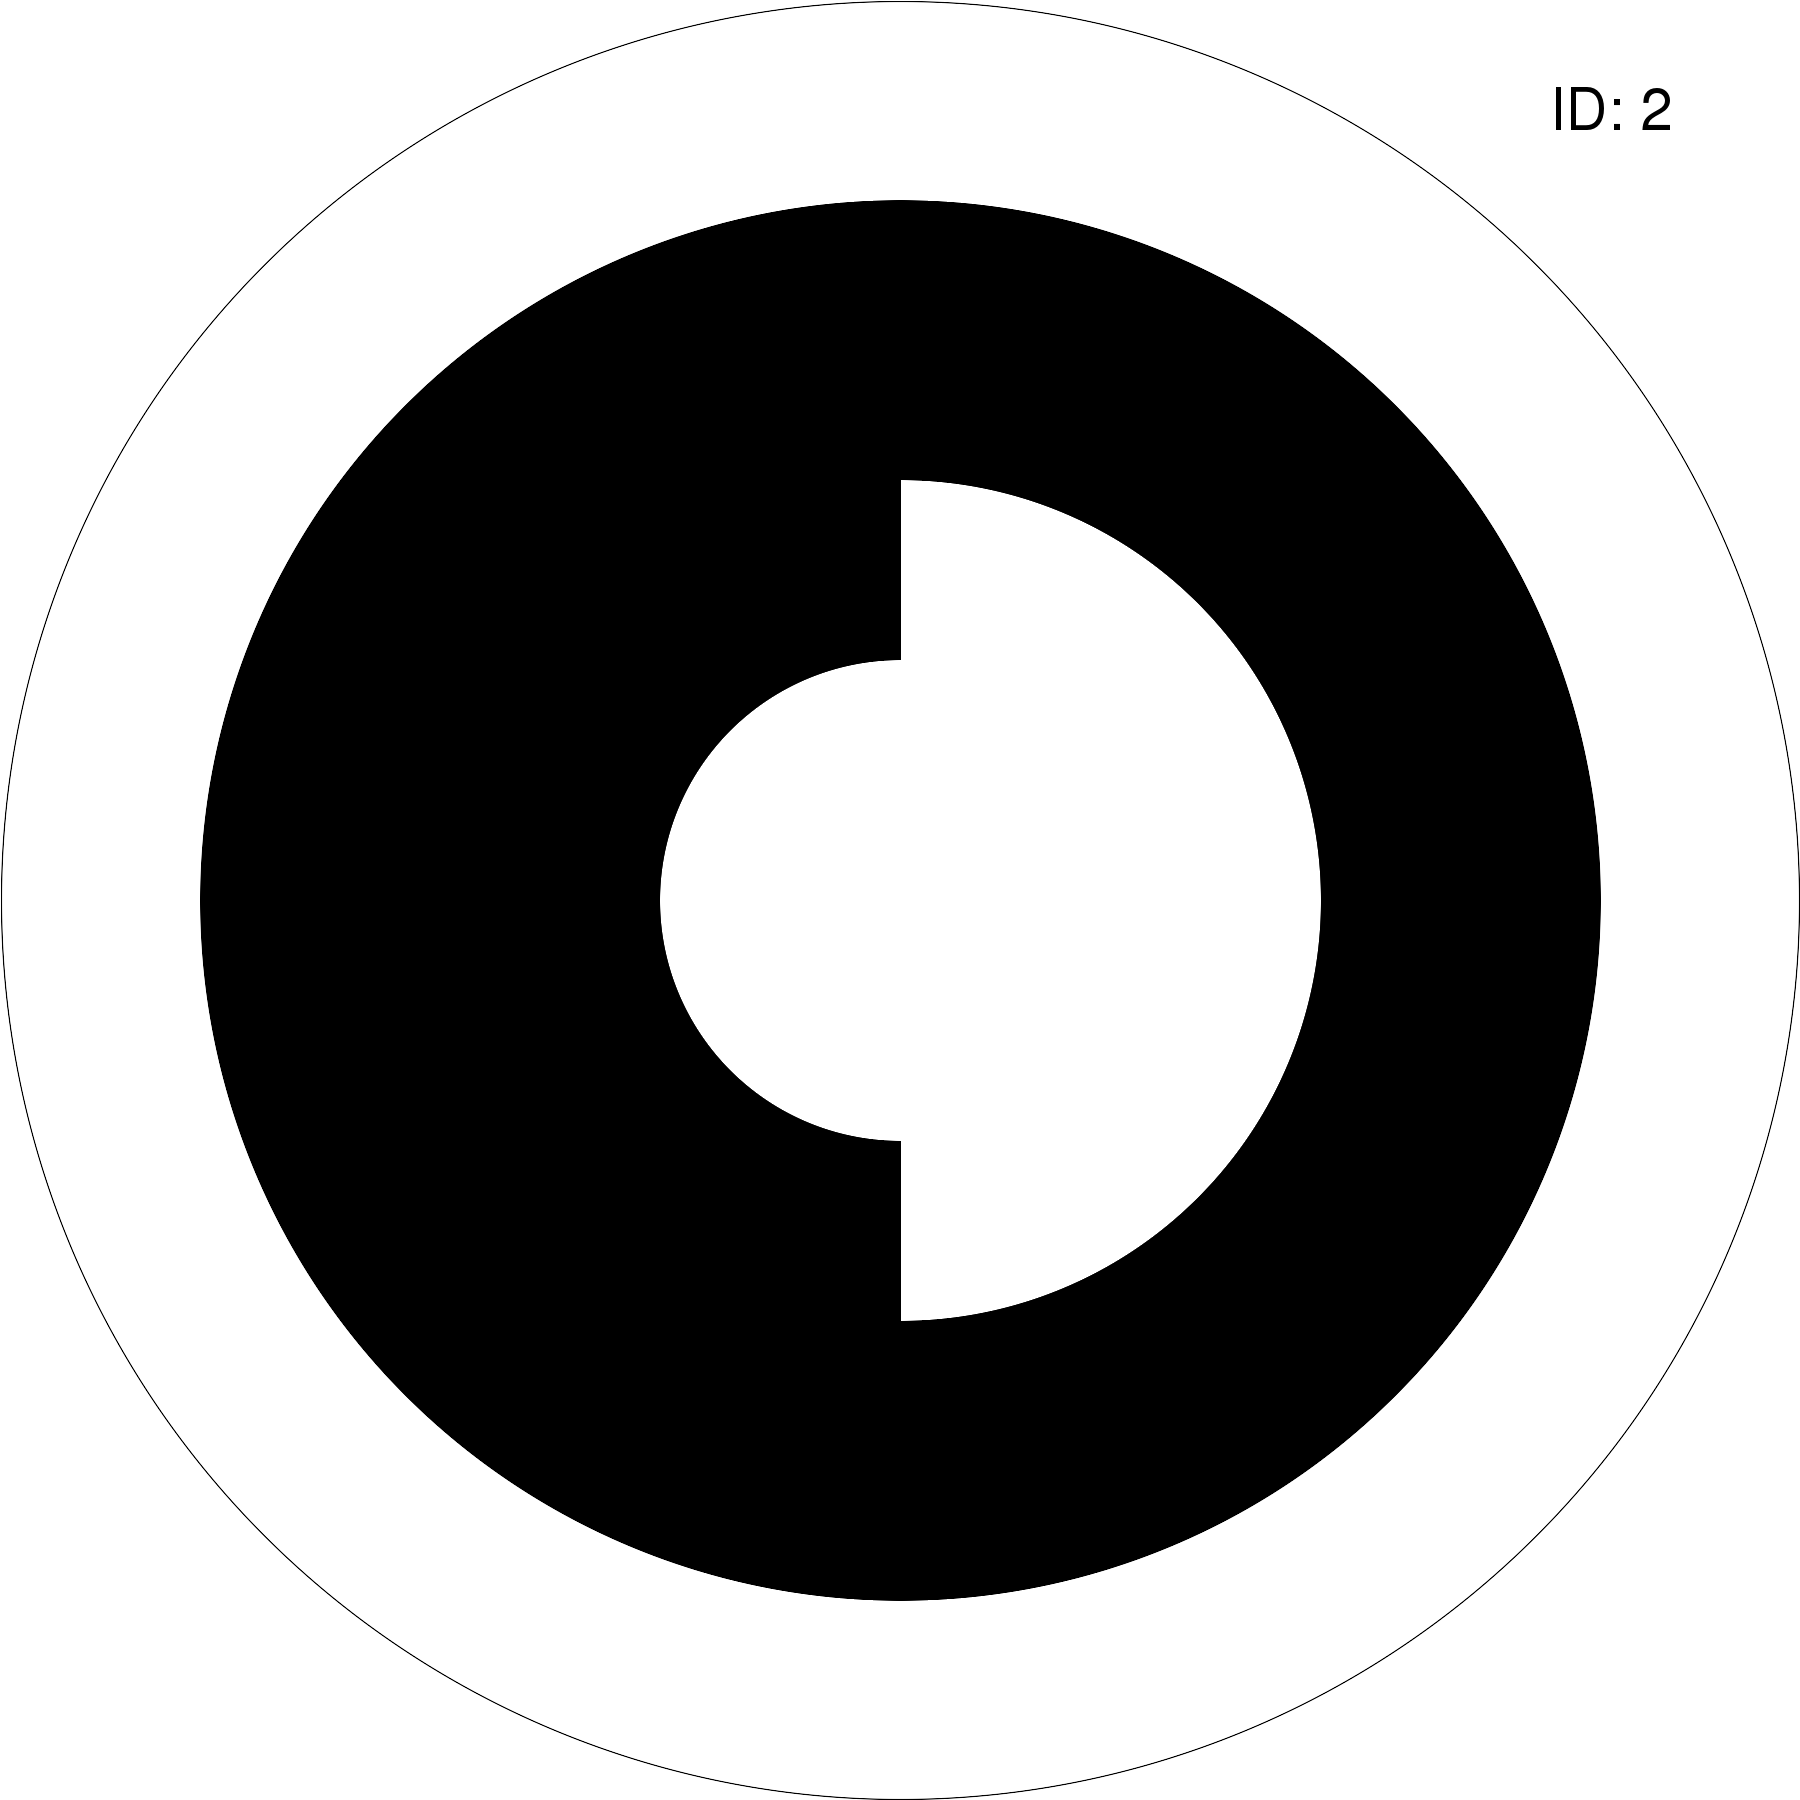
\includegraphics[width=0.2\textwidth]{images/00000002.png}
    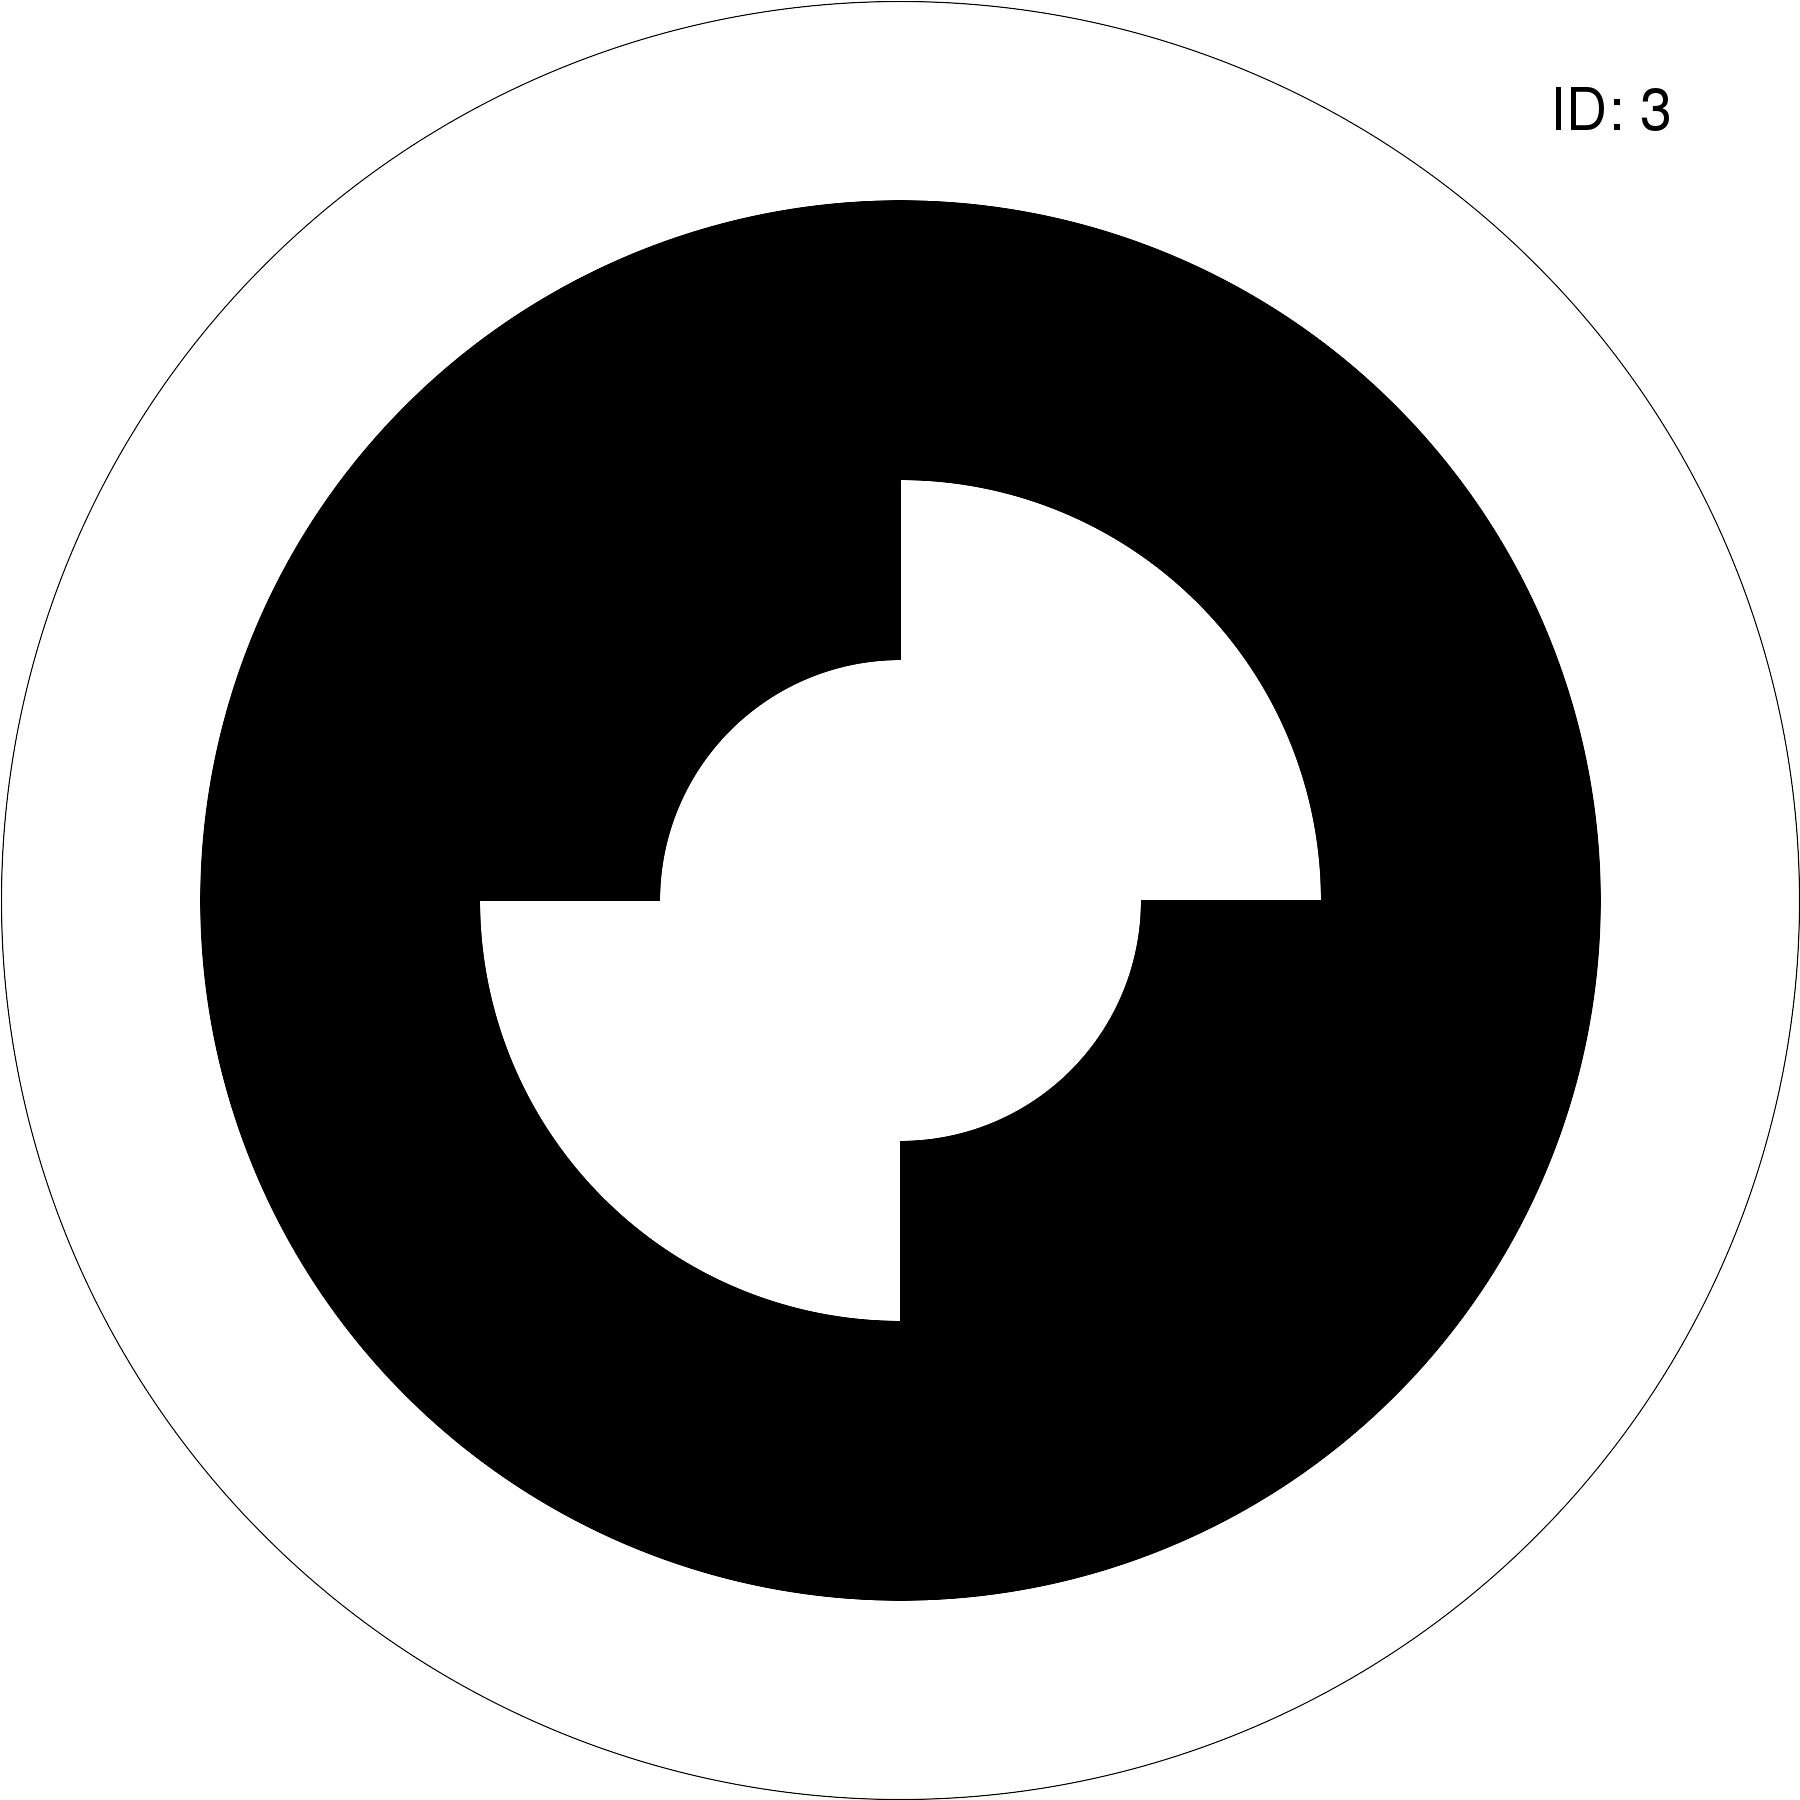
\includegraphics[width=0.2\textwidth]{images/00000003.png}
    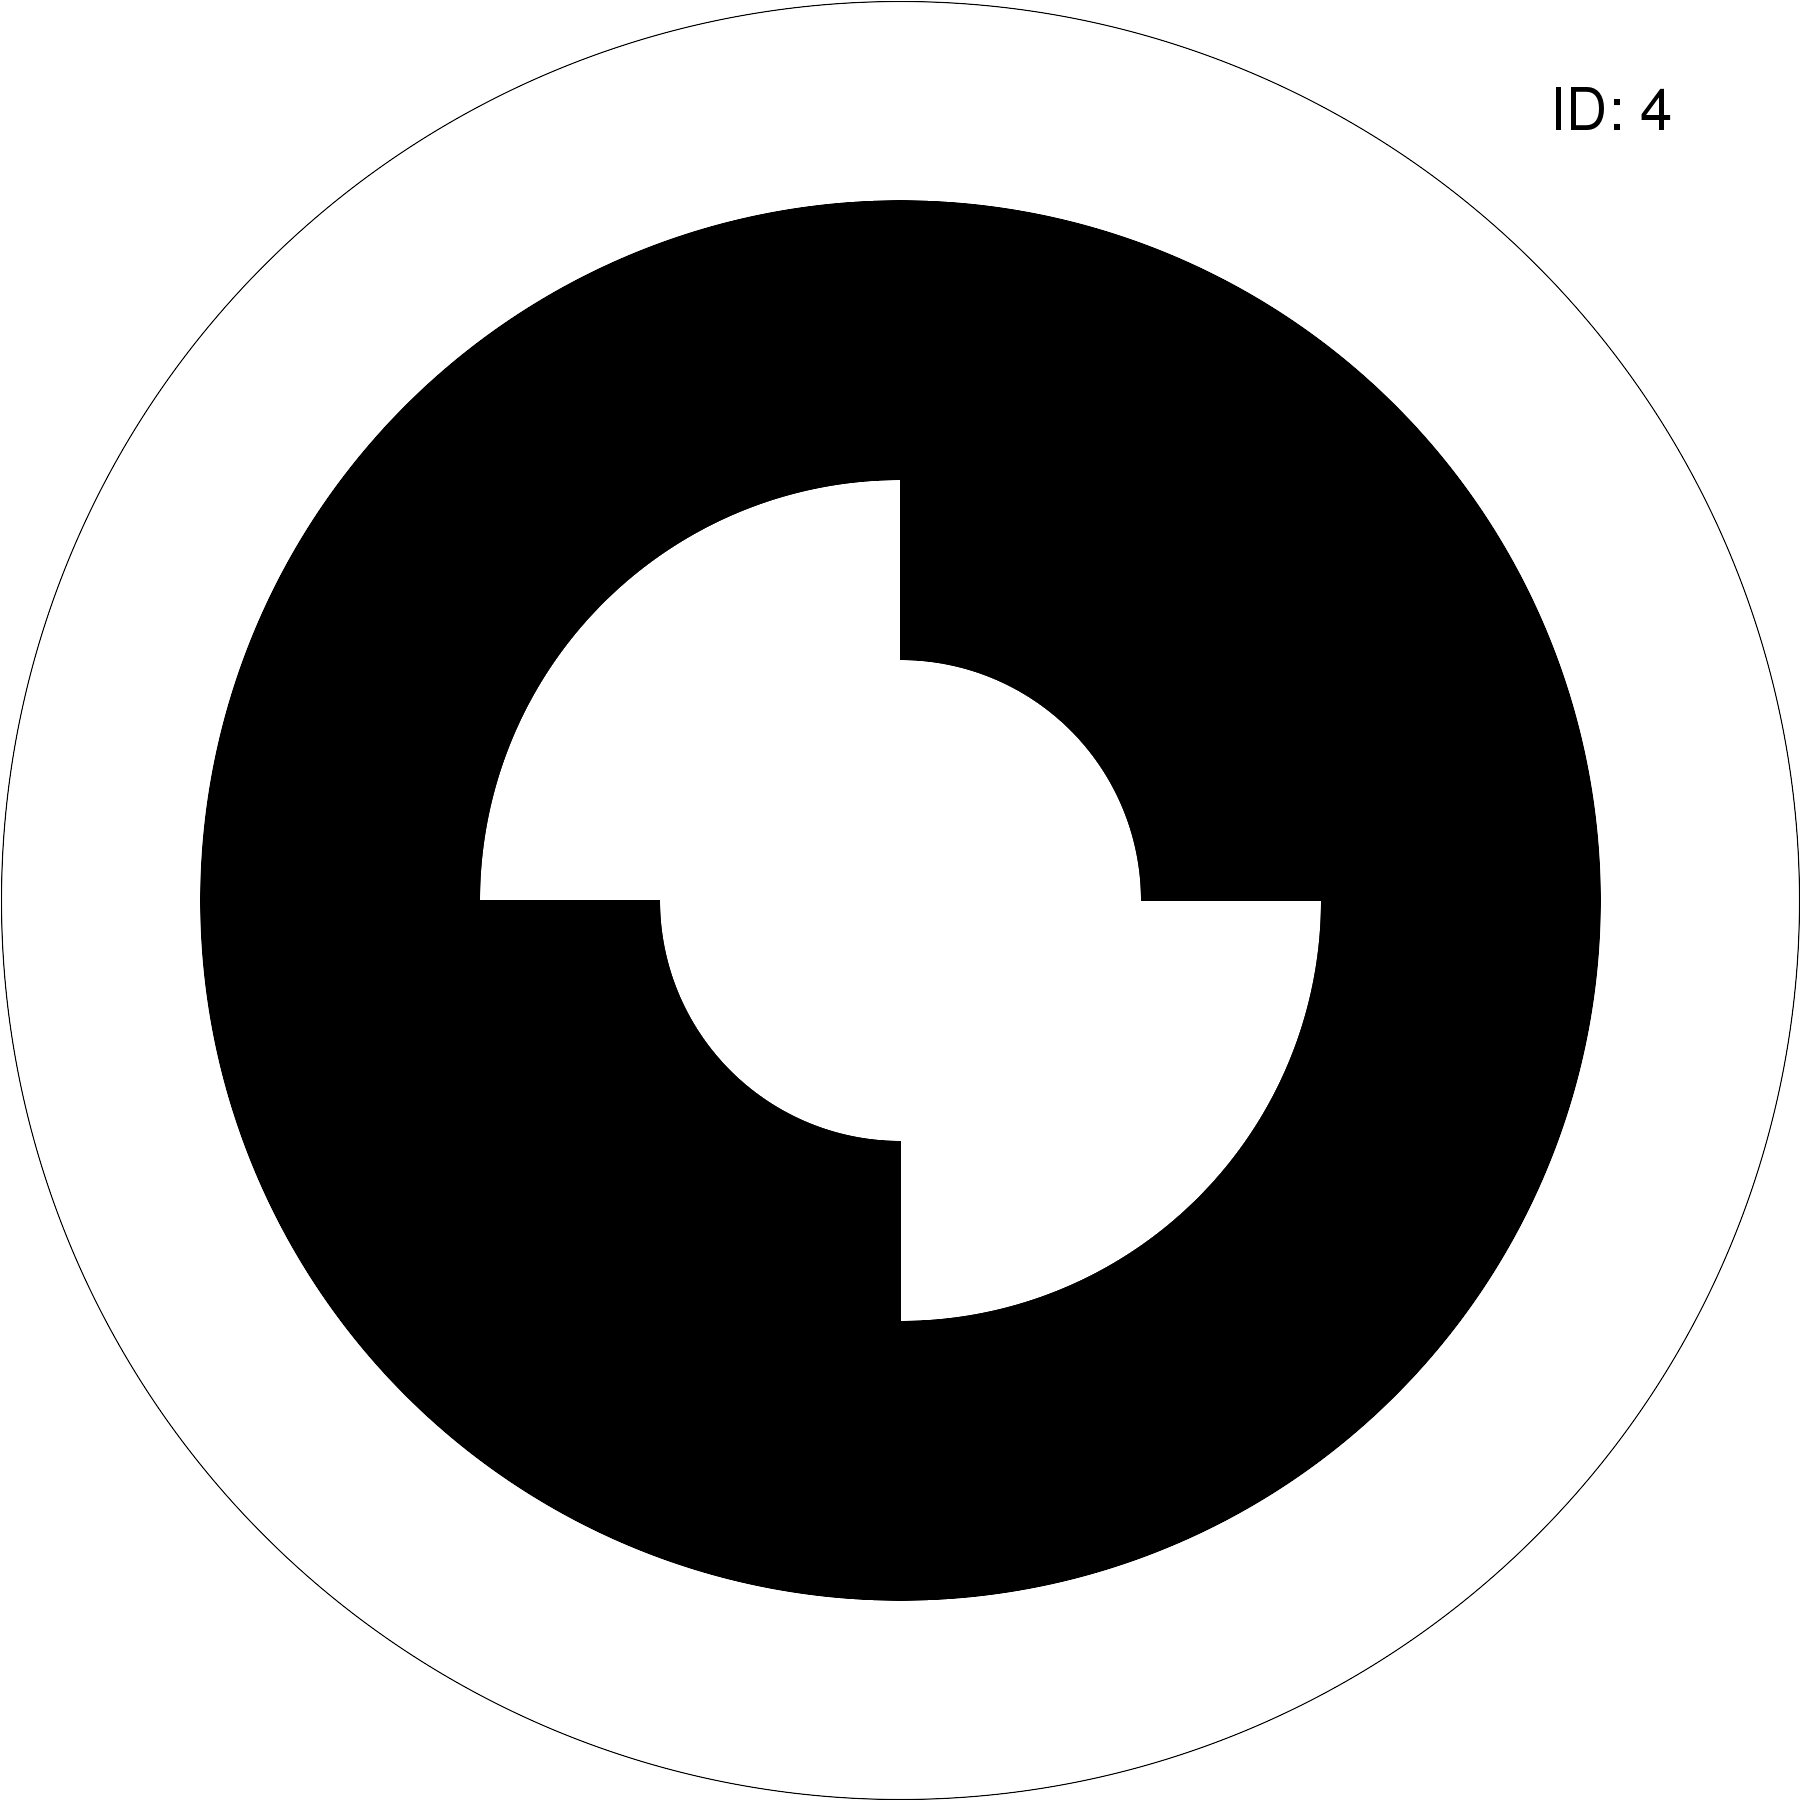
\includegraphics[width=0.2\textwidth]{images/00000004.png}
    \caption{Rotational symmetry in 2-bit WhyCode markers.}
    \label{fig:rotationally_symmetric_whycode_markers}
\end{figure}

\subsection{Orientation Ambiguity}

In contrast to the accurately/unambiguously recognizeable position of WhyCode markers, the orientation
is ambiguous in many circumstances, as can be seen in Figure \ref{figure:orientation_flipping},
particularly during time $t \in [4,8]$.
This ambiguity comes from the fact that the orientation is principally calculated from the semi-axes of the
marker's ellipses under the assumption that the marker is truly a circle.
Calculating the orientation based on these semi-axes gives \textit{two} candidate solutions
that satisfy the assumption that the marker is facing the camera,
and it is difficult to determine which of these candidates represents reality,
especially when the marker is normal or near-normal to the camera's field of view.
The original WhyCode software~\cite{LCAS_whycon} arbitrarily chooses the first solution as correct,
and as such it does not need much analysis except to say that it has a high likelihood of choosing the wrong solution.

In the context of fiducial-based drone landing, the issue of orientation ambiguity affects a drone's ability to
estimate its own pose when its camera is mounted on a gimbal.
Many gimbals do not output their orientations to the flight controller, and their orientations cannot be directly
calculated from control signals in many cases, since many gimbals have sophisticated control systems.
While a control signal may communicate a \textit{target} orientation,
many gimbals have their own IMU and take into account angular motion and acceleration in addition to a control signal.
Therefore, it is difficult to determine the orientation of the gimbal simply based on its control signals.
Without the orientation of either the fiducial marker \textit{or} the gimbal, more assumptions about
the landing scenario are required, such as (for example) that the camera is facing directly down always.

When a drone uses a fiducial marker to determine its position with respect to a landing pad without the assumption
that its camera is in a fixed orientation, it can (theoretically) use the marker's perceived orientation instead.
The drone can rotate the marker's \textit{position} by the inverse of its \textit{orientation} in order to determine
its own position in the reference frame of the marker.
However, such transformations, which depend on the ambiguous orientation of the marker, also exhibit such ambiguities -
discontinuities in the orientation ultimately result in discontinuities in the perceived location of the drone.

\begin{figure}
    \centering
    \begin{subfigure}[b]{0.49\textwidth}
         \centering
         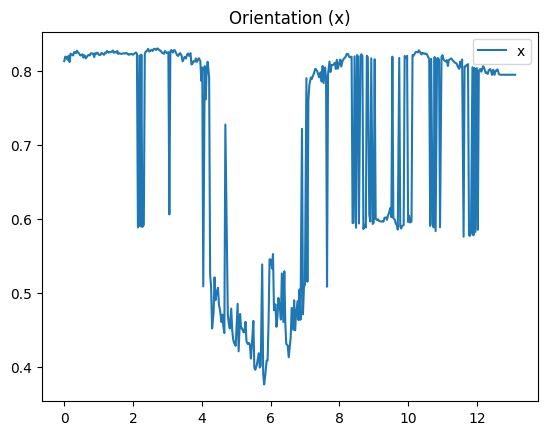
\includegraphics[width=\textwidth]{images/orientation_x_figure.png}
    \end{subfigure}
    \hfill
    \begin{subfigure}[b]{0.49\textwidth}
         \centering
         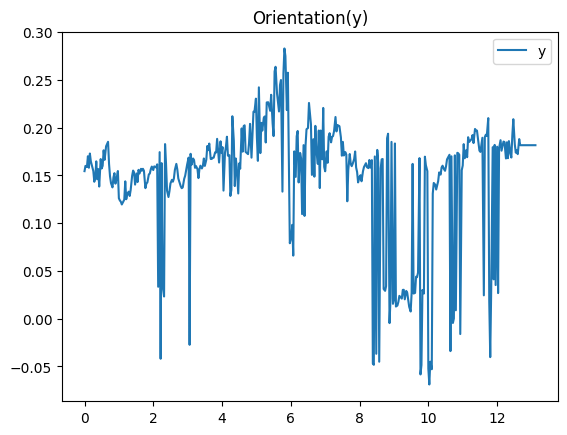
\includegraphics[width=\textwidth]{images/orientation_y_figure.png}
    \end{subfigure}
    \hfill
    \begin{subfigure}[b]{0.49\textwidth}
         \centering
         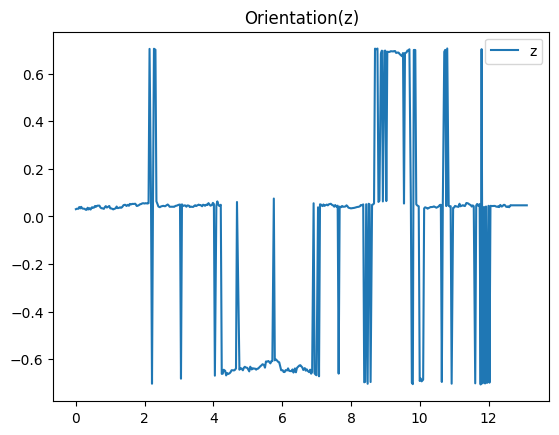
\includegraphics[width=\textwidth]{images/orientation_z_figure.png}
    \end{subfigure}
    \hfill
    \begin{subfigure}[b]{0.49\textwidth}
         \centering
         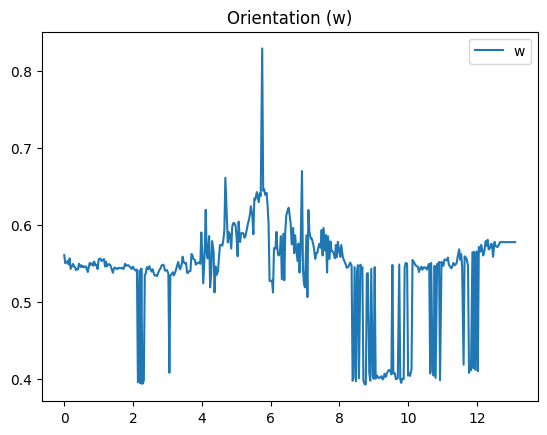
\includegraphics[width=\textwidth]{images/orientation_w_figure.png}
    \end{subfigure}
    \caption{Components of the orientation quaternion for a WhyCode marker. Emphasis is placed on the discontinuities in all components, and sign flipping in the Z component.}
    \label{figure:orientation_flipping}
\end{figure}

Refinements of the WhyCon/WhyCode software, such as that proposed by Jiri Ulrich~\cite{julrich_whycon} (shown in ) attempt to disambiguate
the orientation, with partial success.
This method assumes that all ``teeth'' that form the marker's ID should have the same number of sample points,
and therefore chooses the candidate solution that has lower variance of the number of sample points per tooth.
The samples are collected along the ellipse that is halfway between the white and black ellipses of the marker.
The candidate solutions predict this ellipse to be in slightly different places,
owing to the distortion caused by the camera lens.
The rationale for the method is that the correct solution should predict the ellipse to be in its correct place,
minimizing the variance in the number of sample points that coincide with each tooth.
Conversely, the incorrect solution should predict the ellipse to be in the incorrect place,
and therefore fewer sample points should coincide with teeth one side, increasing the variance.
This provides a baseline on which to disambiguate the solutions, but does not reliably choose the correct one,
especially as the candidate solutions get closer and closer and the marker becomes more and more normal to the camera.

\begin{figure}
    \centering
    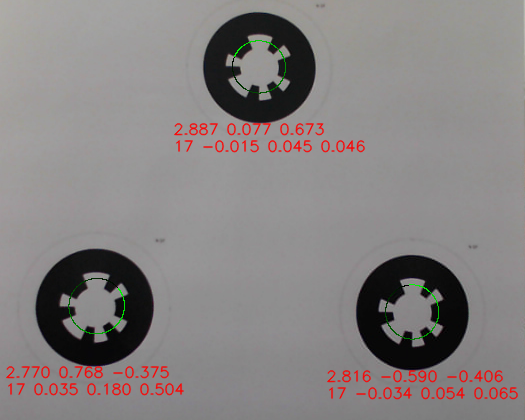
\includegraphics[width=0.5\textwidth]{images/cropped_whycode_3_8_jiri_example}
    \caption{Example from Jiri Ulrich's code, showing the circular sampling locations.}
    \label{figure:jiri_whycode}
\end{figure}

\begin{figure}
    \centering
        \begin{subfigure}[b]{0.49\textwidth}
         \centering
         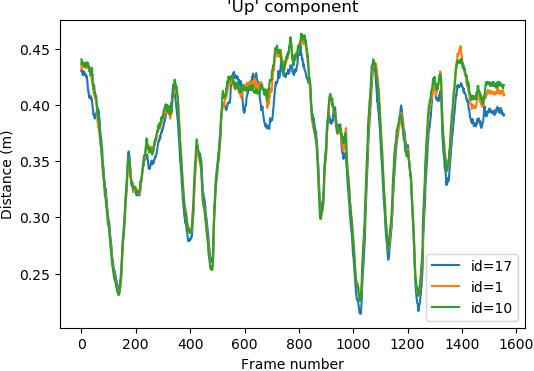
\includegraphics[width=\textwidth]{images/jiri.csv_figure_u}
    \end{subfigure}

    \begin{subfigure}[b]{0.49\textwidth}
         \centering
         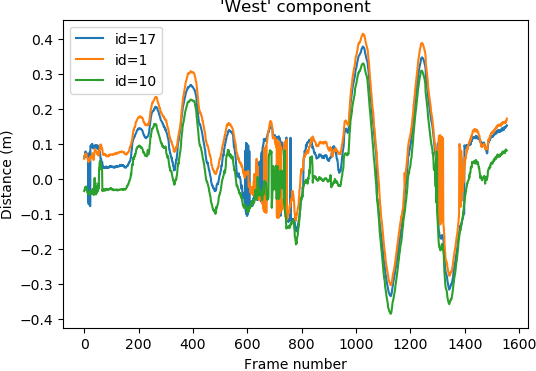
\includegraphics[width=\textwidth]{images/jiri.csv_figure_w}
    \end{subfigure}
    \hfill
    \begin{subfigure}[b]{0.49\textwidth}
         \centering
         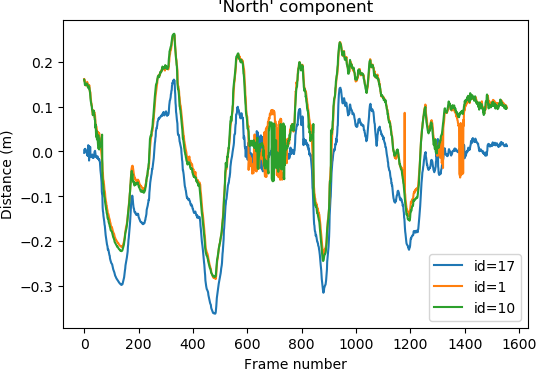
\includegraphics[width=\textwidth]{images/jiri.csv_figure_n}
    \end{subfigure}

    \caption{Each of the components of the perceived camera translation for 8-bit WhyCode markers with IDs 1, 10, and 17, using Jiri Ulrich's decision metric.
    The discontinuities occur mostly in the "west" and "north" components between frames 600 and 800, but also between frames 1200-1400.}
    \label{figure:jiri_uwn}
\end{figure}

\subsection{Proposed Solutions}

As part of this project, I explore two different ways of solving the orientation ambiguity.

\subsubsection{Radial Tooth Edge Sampling}

The first method (the \texttt{ellipse\_sampling} branch of ~\cite{uzgit_whycon}) is similar to that proposed by Jiri Ulrich,
in that it is based on decreasing variance in sample points along the teeth.
After the two candidate solutions for the orientation and the marker ID have been determined,
a second phase of sampling begins.
Each candidate solution predicts the center of the inner, white circle in pixel coordinates.
(Since this system is designed to be lightweight, the center is not actually calculated, nor needed, to determine the position of the marker,
and explicit calculation of this center is neglected by default.)
Given the structure of WhyCode markers, we can assume that the circle along which the ID is sampled
has a radius of $1.5r$, where $r$ is the radius of the inner circle, and the radius of the circle bounding the teeth is $2r$.
Further, from the ID sampling, we can identify the angle that goes through the center of each tooth.
This makes it possible to test how well the candidate solution is centered on the marker at many points,
and leverages the fact that camera distortion increases (and therefore prediction errors increase in magnitude) as one moves away from the center of the image.

The method does decrease the number of discontinuities in the perceived camera location, as shown in Figure \ref{figure:ellipse_sampling_uwn},
at the cost of significantly more sample points (more than double the original number).
Unfortunately, it does not eliminate the discontinuities enough to justify the additional computational requirements.

\begin{figure}
    \centering
    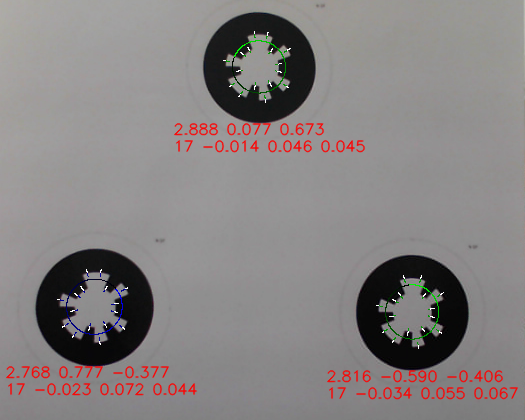
\includegraphics[width=0.5\textwidth]{images/cropped_whycode_3_8_ellipse_sampling_example}
    \caption{Example of sampling WhyCode markers on the radial edges of the teeth.
    The black/blue circle illustrates ID sampling locations, with the bluest samples occurring first, and blackest samples occuring last.
    Each of the blue/white radial line segments illustrates the sampling of the predicted edges of the teeth.
    The method chooses that solution that minimizes the variances of the ratio of blue to white on these line segments.
    }
    \label{figure:ellipse_sampling}
\end{figure}

\begin{figure}
    \centering
        \begin{subfigure}[b]{0.49\textwidth}
         \centering
         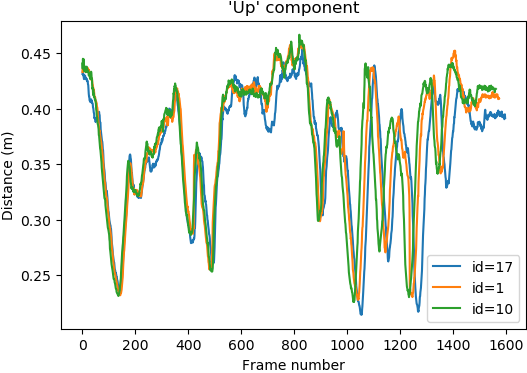
\includegraphics[width=\textwidth]{images/ellipse_sampling.csv_figure_u}
    \end{subfigure}

    \begin{subfigure}[b]{0.49\textwidth}
         \centering
         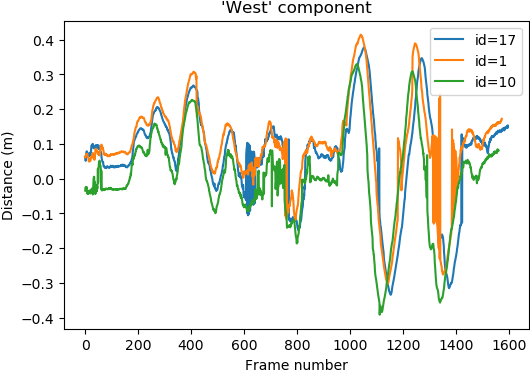
\includegraphics[width=\textwidth]{images/ellipse_sampling.csv_figure_w}
    \end{subfigure}
    \hfill
    \begin{subfigure}[b]{0.49\textwidth}
         \centering
         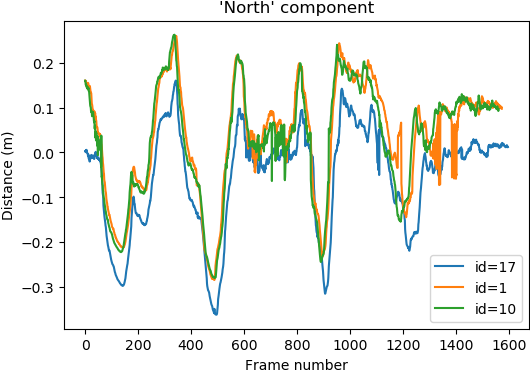
\includegraphics[width=\textwidth]{images/ellipse_sampling.csv_figure_n}
    \end{subfigure}

    \caption{Each of the components of the perceived camera translation for 8-bit WhyCode markers with IDs 1, 10, and 17, using the tooth edge sampling decision metric.
    The discontinuities still occur mostly in the "west" and "north" components between frames 600 and 800, but also between frames 1200-1400.}
    \label{figure:ellipse_sampling_uwn}
\end{figure}

\subsubsection{Co-planar Markers}

The second method works under the assumption that all markers are co-planar.
Since the WhyCode system can accurately and quickly determine the positions of the markers,
this assumption allows the orientation of co-planar markers to be determined unambiguously,
\textit{when 3 or more markers are detected simultaneously}.
For each input image, the WhyCode algorithm identifies all markers and stores their positions.
Additional code assumes that the markers are in a co-planar ``bundle'' and attempts to find the normal vector to the
plane implied by the markers' locations using regression.

This algorithm significantly reduces the number of discontinuities in the perception of the camera location,
as shown in Figure \ref{figure:plane_uwn}.
This comes at the computational cost of performing a regression to calculate the orientation of the plane at each frame.
It also adds additional constraints: at least 3 co-planar (and non-colinear) markers must be visible at all times.
This is problematic with a system such as WhyCode, which does not allow for embedding markers within other markers,
because the required view area increases significantly to accommodate 3 markers simultaneously.

\begin{figure}
    \centering
        \begin{subfigure}[b]{0.49\textwidth}
         \centering
         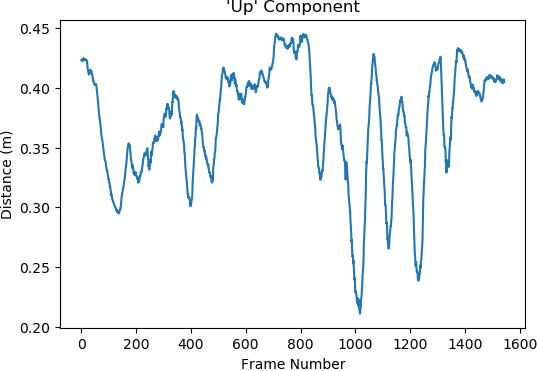
\includegraphics[width=\textwidth]{images/bundles.csv_figure_u}
    \end{subfigure}

    \begin{subfigure}[b]{0.49\textwidth}
         \centering
         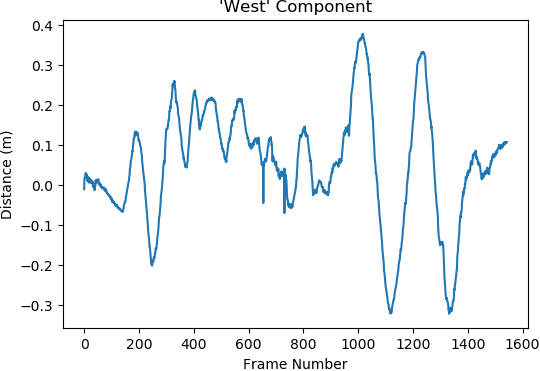
\includegraphics[width=\textwidth]{images/bundles.csv_figure_w}
    \end{subfigure}
    \hfill
    \begin{subfigure}[b]{0.49\textwidth}
         \centering
         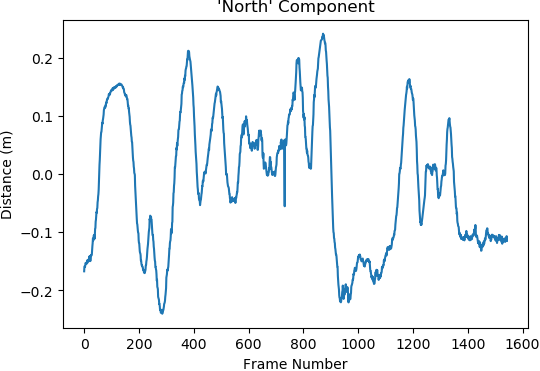
\includegraphics[width=\textwidth]{images/bundles.csv_figure_n}
    \end{subfigure}

    \caption{Each of the components of the perceived camera translation for a ``bundle'' of co-planar 8-bit WhyCode markers with IDs 1, 10, and 17.
    This algorithm significantly reduces the number of discontinuities.}
    \label{figure:plane_uwn}
\end{figure}

\subsection{Conclusion}

WhyCode, though a powerful and computationally efficient fiducial system, is not well-suited to the task of landing a drone with a gimbal-mounted camera.
While the system provides accurate, efficient, and scalable position estimation, the ambiguities and discontinuities in its orientation estimation
prevent the required pose transformations without prohibitively expensive algorithmic extensions or constraints.